\documentclass [a4paper,11pt]{article}

\usepackage[numbers,sort&compress]{natbib}
\usepackage [francais]{babel}
\usepackage[utf8]{inputenc}%       encodage du fichier source
\usepackage[T1]{fontenc}%          gestion des accents (pour les pdf)
\usepackage[a4paper]{geometry}%    taille correcte du papier
\usepackage{hyperref}%			   gestion des hyperliens
\usepackage{graphicx}%			   gestion des images
\usepackage{fancyhdr}%
\usepackage{lastpage}%			   pour avoir le numero de page
\usepackage{fancyvrb}%			   meilleur verbatim
\usepackage{chngcntr}%			   pour numéroté les figures au lieux du numéro de section
\usepackage[toc,page]{appendix}%   pour les annexes
\usepackage{url}

\graphicspath{{img/}} % Chemin par defaut des images
\pagestyle{fancyplain}
\fancyhf{}
\cfoot{\thepage\ sur \pageref{LastPage}}

\begin{document}

\begin{titlepage}
\begin{center}
{\bf Université Sciences et Technologies - Bordeaux1} \vspace{0.5cm}\\

{\bf {\large Master 2 Informatique : Genie logiciel parcours conduite de projet}}\\
%{\emph{Rapport du Projet d'Etude et de Développement }}\\\vspace{1cm}

\begin{figure}[!ht]
  \centering
  
\includegraphics[scale=0.2]{img/uniBx-logo}

  \label{fig:logUniBx}
\end{figure}

{\huge{\bf Visualisation interactive de topologie de plates-formes parallèles avec lstopo et HTML}}\\\vspace{0.5cm}


\end{center}

\textbf{Réalisé par:} Youssef Chagtab, Gregory Emirian, Bertrand Guillozet, Mohamed Labouardy, Clovis Nobile, Ouadii Tabich et Guillaume Verdugo. \\
%\bigskip

\textbf{Responsables:} Philippe Narbel , David Auber.\\

\textbf{Client:} Brice Goglin\\


\end{titlepage}


\tableofcontents

\newpage

\section{Introduction}
Le projet décrit dans ce rapport s'inscrit dans le cadre du projet d'étude et développement du second semestre du Master 2 Informatique.
\newline

Ce projet est lié à \textbf{hwloc} (Hardware Locality) qui est une bibliothèque logicielle exposant de manière portable et abstraite la topologie des machines, en terme de coeurs, caches partagés, threads, sockets, noeuds NUMA, etc \cite{lstopo}.
\newline

Hwloc est notamment utilisée par la plupart des bibliothèques de calcul parallèle de type \textbf{MPI} et \textbf{OpenMP} afin de maîtriser le matériel et ainsi mieux l'exploiter en tenant compte des affinités entre différents composants et entre composants et tâches de calcul.
\newline

L'un des constituants le plus célèbre de hwloc est l'outil \textbf{lstopo} qui permet de visualiser dans de nombreux formats la topologie de la plate-forme telle que analysée par hwloc.
\newline

Le projet était initialement composé de deux parties avec une partie en C et une autre qui utilise les technologies Web. Le but de la première partie était de créer une exportation des données à visualiser tandis que la seconde consistait à implémenter des fonctions d'intéraction.
\newline

Après une première rencontre avec le client, nous avons convenu que la première partie n'était pas nécessaire étant donné que le fichier XML qui peut être généré par hwloc suffisait pour obtenir les données nécessaires à la création de l'application de visualisation. La seconde partie était donc la visualisation des données avec l'ajout d'options pour une personnalisation du rendu final.

\newpage

\subsection{Fonctionnalités}

Les objectifs principaux de ce projet étaient les suivants : \newline

\begin{itemize}
\item extraction de données du fichier XML.
\item visualisation de ces données.
\item implémentation de capacités d'intéraction.
\end{itemize}

La représentation des données issues du fichier XML est sensiblement la même que celle fournie par hwloc. Effectivement le but n'était pas d'avoir une représentation différente de celle produite par la bibliothèque mais d'obtenir la même et de pouvoir l'exploiter dans un navigateur. 
\newline

Cette représentation est essentiellement réalisée en HTML, CSS et Javascript avec notamment l'utilisation de bordures pour définir les contours de chaque objet. Nous reviendrons en détail sur les technologies utilisées dans l'une des parties suivantes.

\begin{figure}[!h]
\centering
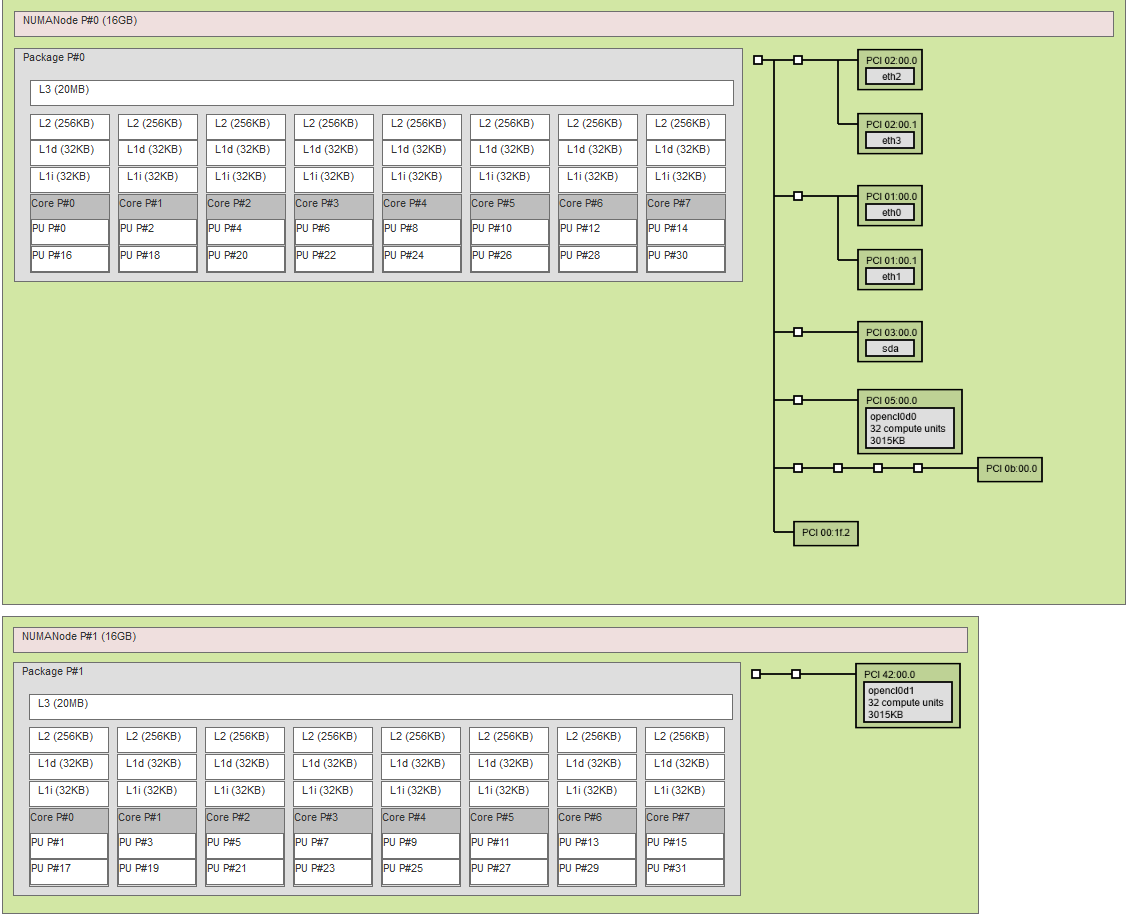
\includegraphics[scale=0.5]{img/alaric.png}
\caption[Résultats]{Exemple de représentation pour le XML Alaric}
\end{figure}

Le second objectif consistait à implémenter des fonctions permettant de personnaliser l'affichage des données issues du fichier XML généré, selon les besoins du client. Voici une liste des principales fonctionnalités d'intéraction : \newline

\begin{itemize}
\item la possibilité de cacher ou de rendre visible certains éléments de la représentation comme les différents caches, la partie PCI ou des entités parentes comme des packages, groupes ou autres afin d'avoir une représentation spécifique ou plus générale.
\item une personnalisation des couleurs pour l'ensemble des objets selon les besoins de l'utilisateur ou des standards mis en place.
\item changer la taille de police pour avoir un affichage plus ou moins important selon la visibilité initiale. 
\item exporter au format PDF ou PNG l'ensemble des représentations personnalisées par le client.
\item la possibilité d'enregistrer sur la machine la configuration des couleurs pour pouvoir la réutiliser plus tard et bien sur la possibilité de charger une configuration préexistante.
\end{itemize}

\begin{figure}[!h]
\centering
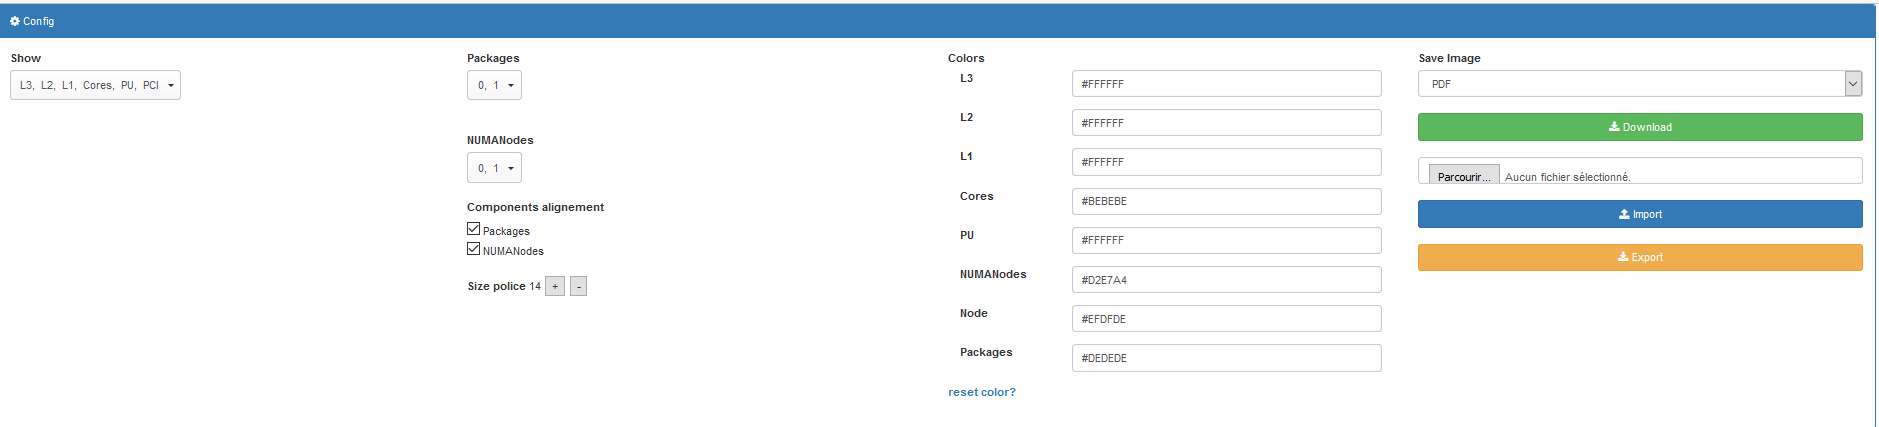
\includegraphics[scale=0.3]{img/filtre.png}
\caption[Résultats]{ Interface graphique du menu d'option }
\end{figure}

\begin{figure}[!h]
\centering
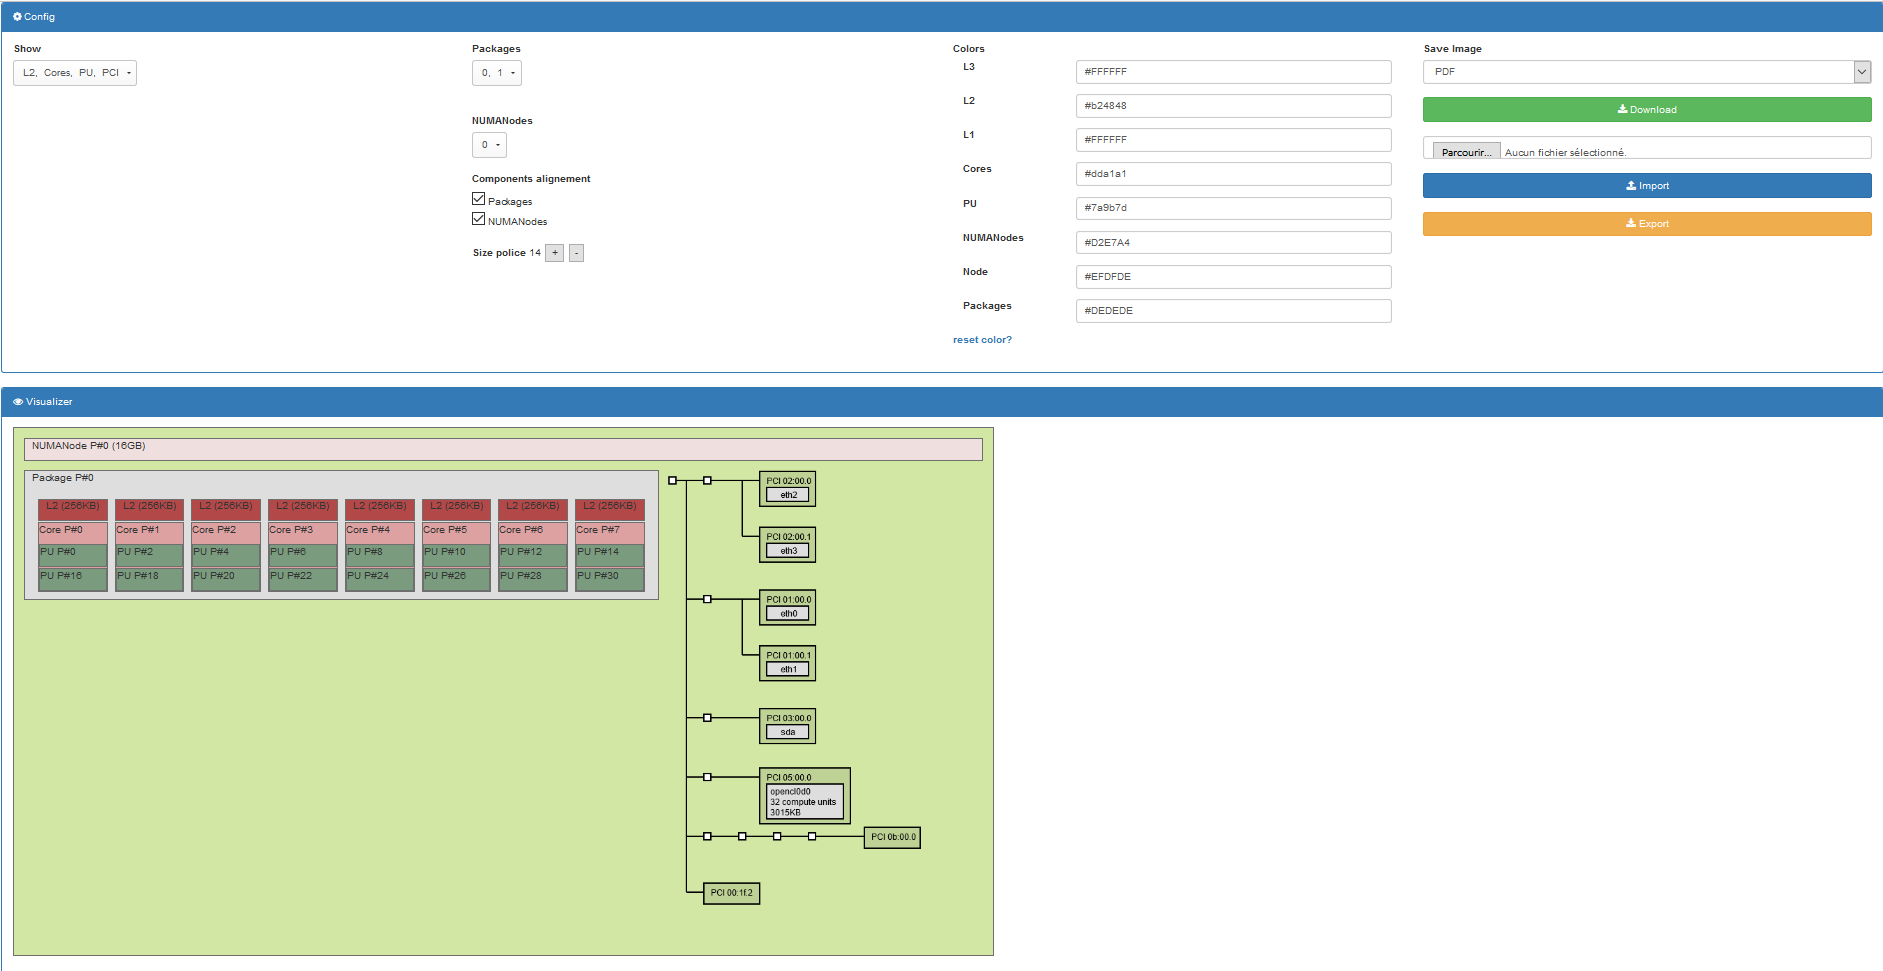
\includegraphics[scale=0.3]{img/alaric_modif.png}
\caption[Résultats]{Exemple de représentation pour le xml Alaric avec options}
\end{figure}

\newpage

\section{Architecture}

\subsection{Technologies utilisées}
\textbf{AngularJS} \cite{angular}, le framework javascript de Google est au cœur des relations entre les vues et les contrôleurs décrits précédemment. L’intérêt principal de cet outil est bien entendu la mise en place d’un architecture \textbf{MVC} et ce, même si l’on ne considère que le côté client d’une application.
\newline

AngularJS étend le \textbf{HTML} classique via l’apport de directives natives qui ont la forme d’attributs HTML et qui permettent de manipuler le \textbf{DOM}. Par exemple, à l’aide de la directive \textbf{ng-repeat} dans components.html on va pouvoir itérer indirectement sur les éléments parents du fichier XML de base (des packages ou des groupes par exemple) et appliquer de façon récursive un même template HTML sur les éléments enfants \cite{Foster14}.
\newline

La visualisation concernant la partie des caches et des cœurs s’appuie sur du HTML via des balises \textbf{div} et \textbf{span} aidées par des feuilles de style \textbf{CSS}.

\newpage

\begin{figure}[!h]
\centering
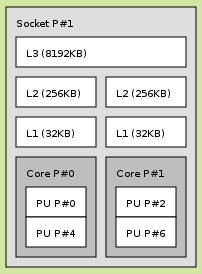
\includegraphics[scale=0.5]{img/caches.png}
\caption[Résultats]{Exemple d'une représentation des caches et des coeurs obtenue avec lstopo}
\end{figure}

Pour la partie concernant les PCI il a fallu essayer plusieurs outils avec des résultats très variables. 

\begin{figure}[!h]
\centering
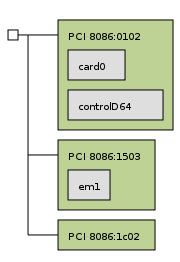
\includegraphics[scale=0.5]{img/treePCI.png}
\caption[Résultats]{Exemple d'un arbre PCI obtenu avec lstopo}
\end{figure}

Voici les principales technologies qui ont été testées pour se rapprocher au maximum d’un résultat satisfaisant :
\newline

\begin{itemize}
 \item La bibliothèque graphique javascript \textbf{D3.js} spécialisée dans la représentation de données sous forme graphique et dynamique \cite{d3}.
 \item La bibliothèque javascript \textbf{JointJS} qui permet la création de diagramme interactif \cite{jointjs}.
 \item Le composant HTML \textbf{canvas} qui permet la réalisation de dessins \cite{canvas}.
 \newline
\end{itemize}

Dans le cas de D3, en utilisant un modèle surtout destiné à la représentation d’arborescence de fichiers \cite{Bostock16} nous sommes parvenus à un résultat proche de celui attendu. La principale différence résidait dans la représentation des entités PCI qui n’était pas exactement la même que celle de référence.
\newline

Avec JointJS nous étions également parvenus à un résultat satisfaisant. Cette fois la différence se faisait dans la représentation des arêtes ou des branches qui n’étaient pas tout à fait conforme aux attentes.
\newline

Si les solutions avec ces deux outils ont été abandonnées, malgré le fait qu’elles permettaient une interaction, c’est parce que les deux différentes représentations que l’on obtenait était gravement déformées lors de l’exportation en PNG (une fonctionnalité importante de l’application). Tandis que les branches étaient transformées en polygone pleins, les entités étaient dépourvues de contour. 
\newline

Ces deux bibliothèques utilisent la technologie \textbf{SVG} (Scalable Vector Graphics) pour la représentation des données. Or cela implique une conversion avec canvas avant de pouvoir être exporté sous un format d’image. C’est sans doute cette conversion qui posait problème mais n’ayant pas trouvé de véritable solution nous nous sommes tourné vers la troisième technologie : canvas.
\newline

Canvas est un composant qui fait partie de la spécification \textbf{HTML5} et qui correspond à une zone de dessin. Du code javascript permet ensuite d’accéder à cette zone et d’utiliser toute une série de fonctions de dessin comme une \textbf{API} classique.
\newline

L’interface graphique de l’application utilise l’outil \textbf{Bootstrap} et plusieurs directives AngularJS particulières :
\newline

\begin{itemize}
 \item \textbf{angular-bootstrap-colorpicker} pour une sélection poussée des couleurs sur chaque élément \cite{colorpicker13}.
 \item \textbf{angular-multi-select} pour une liste déroulante des éléments à afficher ou non \cite{select14}.
 \newline
\end{itemize}

La conversion du fichier XML en JSON pour une manipulation des données en JavaScript est possible grâce à la bibliothèque \textbf{x2js} qui présente l’intérêt de ne pas avoir de dépendances \cite{x2js14}.
\newline

\subsection{Système MVC}
L’image ci-dessous réalisée avec le logiciel \textbf{Enterprise Architect} représente un schéma de l’architecture de l’application. Il est important de comprendre que ce schéma n’utilise pas une norme ni même un langage de modélisation en particulier. Il a simplement été conçu pour simplifier la compréhension et les liens existants entre les différentes entités de l’application, il ne peut être considéré comme exactement conforme à la réalité.
\newline

\begin{figure}[!h]
\centering
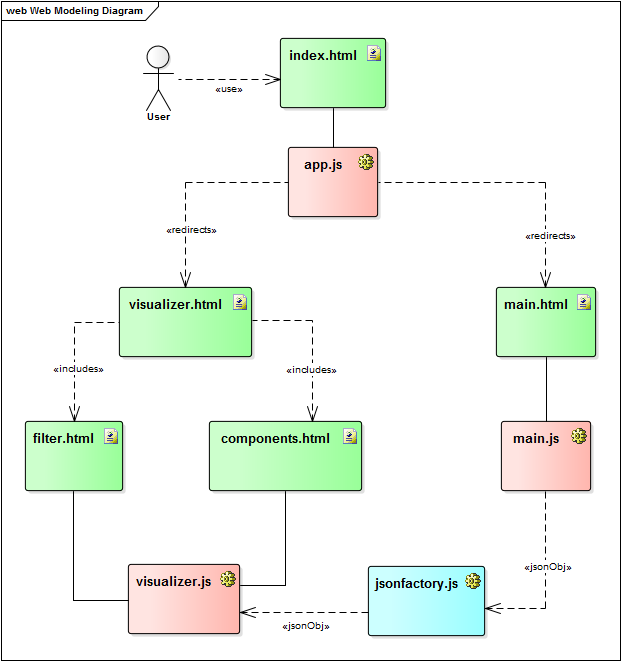
\includegraphics[scale=0.5]{img/ped_architecture.png}
\caption[Résultats]{Architecture simplifiée de l'application}
\end{figure}

D’une certaine façon l’application est organisée suivant une architecture modèle-vue-contrôleur avec quelques particularités. Dans un souci de lisibilité, le schéma utilise un système de couleurs. En vert sont représentées les vues qui, dans notre cas, correspondent à des fichiers HTML et en rouge les différents contrôleurs.\newline

%Lors de la création du site web, nous avions utilisé une architecture \textbf{monopage} (single-page application) avec Angular Js, c'est à dire une application web accessible via une page web unique, contrairement à un site web classique composés de plusieurs pages et donc de plusieurs codes sources. Cette architecture nous permet de naviguer sur le site de la même manière qu'un site web classique mais sans avoir à recharger notre page à chaque action demandée, plus précisément les liens ne rechargent pas la page mais le contenu est modifié au fur et à mesure selon les requêtes. Pour ce faire il existe deux manières differentes: soit on charge tout les éléments dans un fichier html (template), soit on récupere et affiche dynamiquement les ressources nécessaires selon les requêtes envoyées par l'utilisateur.
  
Avant de rentrer plus en détail, il est nécessaire de faire le point sur les objectifs des différentes entités présentes sur le schéma :
\newline

\begin{itemize}
 \item \textbf{index.html} et \textbf{app.js} sont en charge du routage.
 \item \textbf{main.html} et son contrôleur \textbf{main.js} sélectionnent, récupèrent et traduisent les données du fichier XML.
 \item \textbf{visualizer.html}, \textbf{filter.html}, \textbf{components.html} et leur contrôleur visualizer.js affichent et permettent d’interagir avec les données issues du fichier XML.
 \item \textbf{jsonfactory.js} en bleu est un service qui transmet les données issues du fichier XML entre les deux contrôleurs décrits précédemment.
 \newline
\end{itemize}

L’utilisateur accède à l’application via index.html qui est le layout général. Cette page associée au script app.js gère le système de routage de l’application et va insérer le bon template (main.html ou visualizer.html) en fonction de l’URL demandée et en particulier des ancres \cite{Landazuri16}.
\newline

Dans notre cas, il n’existe pas de choix à proprement parler. Lorsque l’utilisateur lance l’application il est forcément dirigé sur main.html qui est la vue en charge de sélectionner le fichier XML à analyser. Le contrôleur associé main.js va traduire ce fichier XML au format JSON et insérer toutes les informations dans une variable javascript qu’il va transmettre au service jsonfactory.js en vue d’être exploitée par le contrôleur visualizer.js.
\newline

La vue visualizer.html inclu deux fragments externes HTML. Le premier, filter.html décrit l’interface graphique avec les différents boutons et autres éléments sur lesquels l’utilisateur peut interagir. Le second n’est autre que components.html qui est la vue pour l’affichage des informations provenant indirectement du fichier XML.
\newline

Ces vues sont en relation avec le script visualizer.js qui contient deux contrôleurs. Le premier contient plusieurs types de fonctions :
\newline

\begin{itemize}
 \item Les fonctions permettant d’extraire les données considérées par l’application et contenues jusqu’alors dans la variable javascript du service jsonfactory.js décrit avant. Ces données dites « scopes » (AngularJS) serviront donc de modèles.
 \item Les fonctions déclenchées par des évènements utilisateurs et celles appelées en réponse.
 \newline
\end{itemize}

Ce contrôleur est donc en lien avec filtre.html et une partie de components.html.
\newline

Le second contrôleur est entièrement dédié à la partie concernant les cartes d’extension PCI et qui seront visuellement représenté sous la forme d’un arbre. Nous verrons dans une prochaine partie les technologies utilisées pour une telle représentation.
\newline

Une demonstration de notre application web est disponible sur ce lien \cite{APPLI}.

\section{Intégration Continue}

L'intégration continue est une étape importante à mettre en place dans le processus de développement logiciel. Nous parlerons donc ici de cette pratique et des outils utilisés au cours de ce projet.

\begin{center}
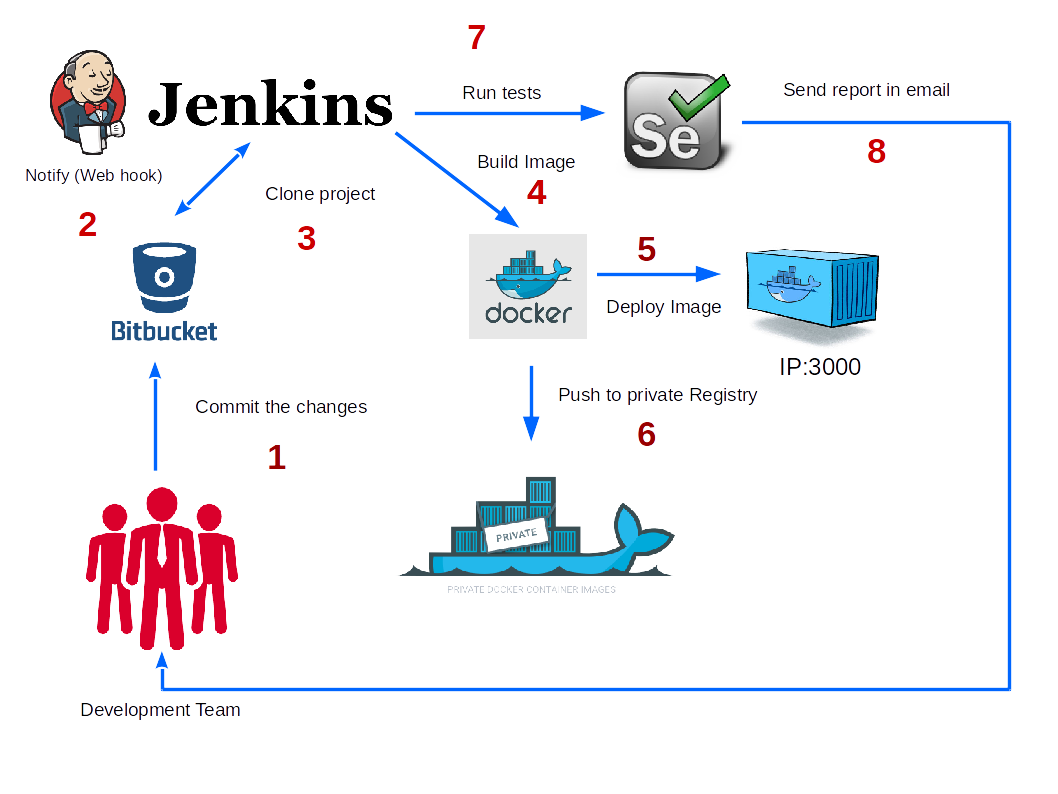
\includegraphics[scale=0.5]{img/ci.png}
\end{center}

Au moment d’un push d’un ou plusieurs commit au niveau de Bitbucket (sur la banche \textbf{release}) on déclenche via un hook la tâche de build qui permet la construction de l'image Docker à partir de Dockerfile, le push de cette image dans un dépôt privé, le déploiement de cette image dans un container exposé sur le port 80 et enfin de passage des tests unitaires au niveau de Jenkins. Dès qu’une modification du code est donc poussée sur le repository, il y a vérification que l’ensemble fonctionne toujours.

\begin{center}
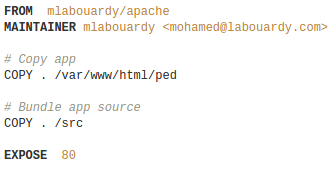
\includegraphics[scale=0.7]{img/Dockerfile.png}
\end{center}

\subsection{Bitbucket}

Un système de versionnement, il a été choisi pour héberger les sources des projets internes et clients.\cite{BITBUCKET} Pour ce projet trois branches ont été utilisé:\newline

\begin{itemize}
 \item \textbf{master} utilisé pour la phase de développement
 \item \textbf{release} utilisé pour la phase de production
 \item \textbf{docs} utilisé pour les documents (rapport, maquettes, cadrage ...)
\end{itemize}

\subsection{Jenkins}

Serveur d'intégration continue, il est capable d’aller se connecter à un outil de gestion de sources (Dans ce cas Git) et de voir si des modifications ont été effectuées. S’il en détecte, il peut lancer un \textbf{build} qui va pouvoir lancer un certain nombre d’actions(déploiement automatisé, tests unitaires ...)

\subsection{Docker}

Docker est un système de container linux ultra léger basé sur les cgroups, lxc et aufs.\newline

L'idée est la suivante pour un build:\newline

\begin{itemize}
 \item Jenkins crée une image docker à partir de Dockerfile
 \item Jenkins push l'image dans un dépot privé
 \item Jenkins crée un container docker à partir de cette image\newline
\end{itemize}

Les containers sont running de manière continue, permettant ainsi aux responsables du projet et au client de tester la dernière version du produit poussé manuellement à partir de Jenkins.

\subsection{Private Registry}

Depot pour stocker l'ensemble des versions de l'application tout au long de la phase de développement

\begin{center}
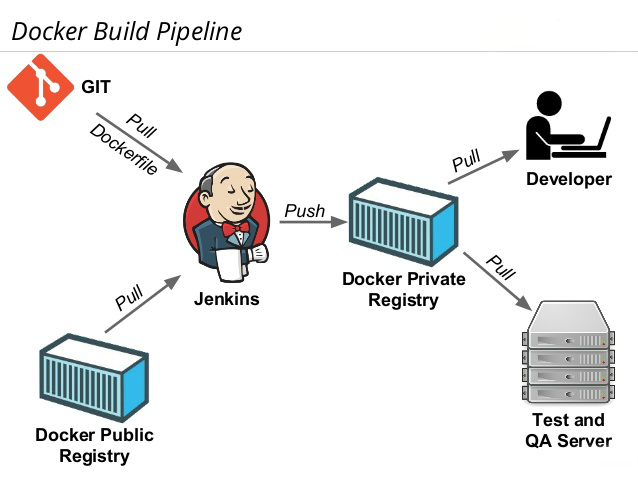
\includegraphics[scale=0.4]{img/registry.png}
\end{center}

L'avatange d'utilisation d'un docker private registry c'est avoir un systéme de versionning pour l'application. et rendre disponible facilement le dernier exécutable.
\subsection{Selenium Webdriver}
WebDriver est un framework de tests fonctionnels issu du projet Selenium, célèbre outil d'automatisation de tests pour navigateurs.\newline

Un exemple des test faites avec l'API Selenium c'est la mesure du temps d'execution pour un ensemble des exemples d'Architecture.

\begin{center}
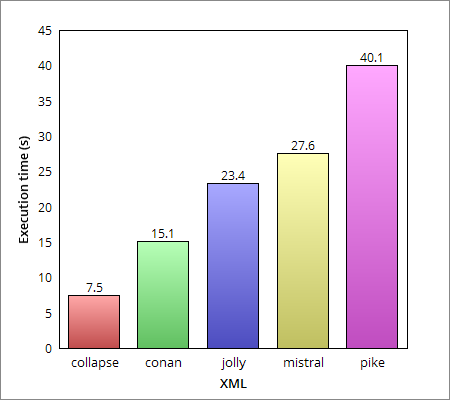
\includegraphics[scale=0.4]{img/benchmark.png}
\end{center}

\subsection{JSLint/CSSLint}

La qualité du code est vitale pour qu'un projet soit pérenne sur le moyen et long terme. De nombreux outils existent pour automatiser les contrôles et générer des rapports statistiques:\newline

\textbf{JSLint} est un analyseur de code Javascript. Son but est de parser le code Javascript pour vérifier que vous respecter les règles de coding Javascript.\newline

\begin{center}
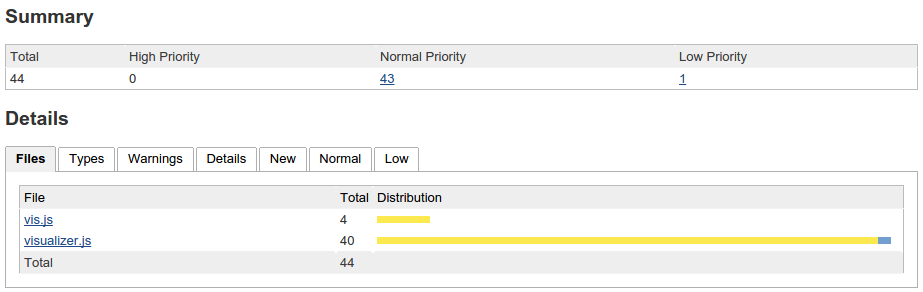
\includegraphics[scale=0.4]{img/checkstyle.png}
\end{center}

\textbf{CSSLint} détecte les problèmes d'une feuille de style CSS.

\begin{center}
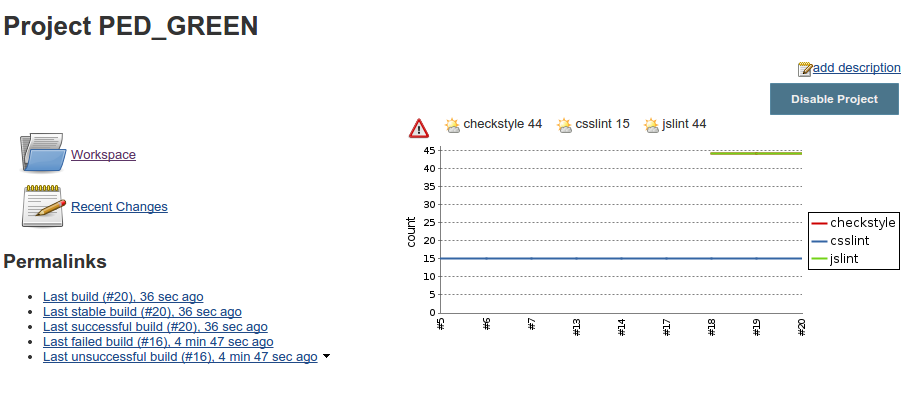
\includegraphics[scale=0.4]{img/jslint.png}
\end{center}

\subsection{AngularJS Batarang}

Afin de développer tester, déboguer et surveiller notre application AngularJS, on a installé un plugin sur le navigateur:\newline

Une extension de Google Chrome. Il permet d'observer le code en action, de faire des benchmarks sur les fonctions, modules, etc...

\newpage
\section{Gestion de projet}

\subsection{Scrum}

Durant l'ensemble du projet nous avons suivi la méthode Scrum qui est une méthode agile. Le but était d'être en conditions réelles de projet avec une équipe de sept personnes. 
\newline

Pour appliquer la méthode Scrum nous avons utilisé le logiciel Icescrum qui permet de répondre aux besoins de ce genre de projet \cite{ICESCRUM}. Il nous a permis notamment de définir un backlog qui contenait l'ensemble des User Stories à réaliser pendant la durée du projet, définir différents sprints avec ces User Stories et les différentes tâches les constituant. 
\newline

Dans chaque sprint on peut définir le kanban pour les différentes tâches et connaitre leur état. Nous avons choisi de réaliser des sprints de deux semaines comme c'était prévu à la base.
\newline

Pour les tâches nous avons choisi différentes couleurs afin de différencier les différents types de tâches :
\newline

\begin{itemize}
\item Tâches jaunes: elles représentent le code produit pour le projet.
\item Tâches bleues: elles représentent les tests de validations pour notre code.
\item Tâches grises et rouges: elles représentent les recherches concernant certaines bibliothèques non mis en place, la rédaction de rapport et d'analyse comlémentaire.
\end{itemize}

\begin{figure}[!h]
\centering
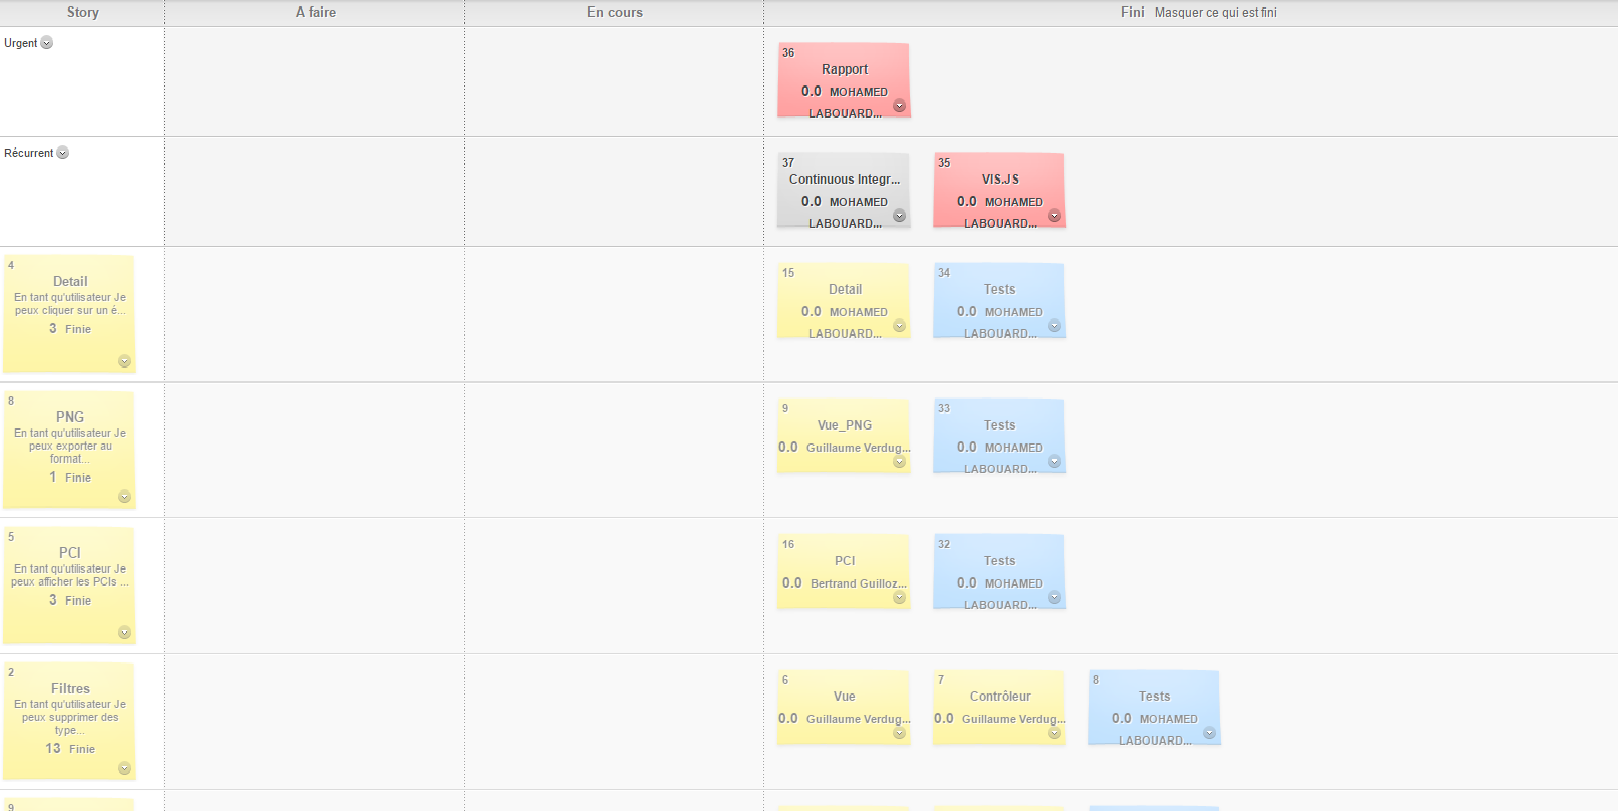
\includegraphics[scale=0.3]{img/icescrum.png}
\caption[Scrum]{Sprint 2 avec les différentes tâches}
\end{figure}

Il est important de noter que les noms apparaissant en dessous des tâches ne correspondent pas forcément au responsable de l'entité. Des rencontres régulière ont eu lieux et une seule personne était chargée de modifier le kanban.

\subsection{Outils complémentaires}
En raison de nombreux problèmes de bug et de ralentissement rencontrés durant tout le projet, nous avons parfois délaissé IceScrum pour créer des kanbans sur des outils différents (Excel). 

\newpage

\section{Critiques}

\subsection{Technologies}
En ce qui concerne les technologies utilisées dans ce projet, nous aurions pu nous tourner vers ReactJS qui est une bibliothèque développée par Facebook et qui permet de manipuler un DOM virtuel.
\newline

Par manque d'expérience avec cette bibliothèque, nous avons choisi de travailler avec AngularJS.

\subsection{Critiques d'IceScrum}
Ce logiciel qui nous a été imposé durant le cycle de développement du projet n'était pas assez d'intuitif et comme nous l'avons évoqué précédemment,des ralentissements liés au serveur nous ont parfois empêchés d'intéragir avec nos sprints.

\subsection{Performances}
On peut trouver plusieurs pratiques qui nous ont permis ou qui pourrait permettre d’améliorer les performances de l’application :
\newline

\begin{itemize}
\item L’utilisation du cache du navigateur qui consiste à garder en mémoire des copies des pages servies. Cela permettra d’éviter la répétition des traitements à chaque fois et gagner au niveau du temps du chargement de la page web.\newline
\item Le \textbf{one time binding} qui permet d’indiquer que le binding ne se fasse qu’une seule fois afin de gagner au niveau performance.
\end{itemize}

\subsection{Améliorations possibles}
Certaines fonctionnalités (non prioritaires) n'ont pas été totalement implémenté tandis que d'autres auraient pu présenter un intérêt : \newline

\begin{itemize}
\item l'exportation en PDF.
\item amélioration des feuilles de style
\item amélioration des arbres PCI qui ne prennent pas en compte toutes les configurations possibles.
\end{itemize}

\newpage

\bibliographystyle{unsrtnat}
\bibliography{report}

\end{document}
